% Author: Izaak Neutelings (February 2020)

\documentclass[border=3pt,tikz]{standalone}
\usepackage{amsmath} % for \dfrac
\usepackage{physics,siunitx}
\usepackage{tikz}
\usetikzlibrary{angles,quotes} % for pic (angle labels)
\usetikzlibrary{arrows.meta}
\usetikzlibrary{calc}
%\usetikzlibrary{decorations.markings}
\tikzset{>=latex} % for LaTeX arrow head
\usepackage{xcolor}
\colorlet{Ecol}{orange!90!black}
\colorlet{Icol}{blue!50!black}
\colorlet{Ccol}{orange!90!black}
\colorlet{Rcol}{green!50!black}
\colorlet{Lcol}{violet!90}
\colorlet{myblue}{blue!70!black}
\colorlet{myred}{red!70!black}
\tikzstyle{Rline}=[Rcol,thick]
\tikzstyle{gline}=[Rcol,thick]
\tikzstyle{bline}=[myblue,thick]
\tikzstyle{rline}=[myred,thick]
\tikzstyle{width}=[{Latex[length=5,width=3]}-{Latex[length=5,width=3]},thick]
\tikzstyle{vector}=[->,very thick]
\tikzstyle{-sm}=[-{Latex[length=3,width=2]}]
\tikzstyle{sm-}=[{Latex[length=3,width=2]}-]
\def\tick#1#2{\draw[thick] (#1) ++ (#2:0.03*\ymax) --++ (#2-180:0.06*\ymax)}
\newcommand\EMF{\mathcal{E}}
\newcommand\VR{\vb{V}\!_R}
\newcommand\VC{\vb{V}\!_C}
\newcommand\VL{\vb{V}\!_L}
\newcommand\IR{\vb{I}_R}
\newcommand\IC{\vb{I}_C}
\newcommand\IL{\vb{I}_L}
\def\xmin{1.8}
\def\xmax{2.0}
\def\ymax{1.8}
\def\ang{35}

\newcommand\rightAngle[4]{
  \pgfmathanglebetweenpoints{\pgfpointanchor{#2}{center}}{\pgfpointanchor{#3}{center}}
  \coordinate (tmpRA) at (\pgfmathresult+45:#4);
  \draw[white,line width=0.6] ($(#2)!(tmpRA)!(#1)$) -- (tmpRA) -- ($(#2)!(tmpRA)!(#3)$);
  \draw[blue!40!black] ($(#2)!(tmpRA)!(#1)$) -- (tmpRA) -- ($(#2)!(tmpRA)!(#3)$);
}


\begin{document}



% PHASOR
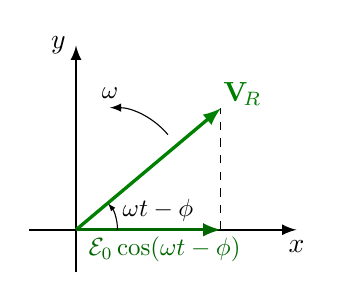
\begin{tikzpicture}
  \def\R{2.4}
  \def\ang{40}
  \coordinate (O) at (0,0);
  \coordinate (X) at (1.4*\xmax,0);
  \coordinate (Y) at (0,1.3*\ymax);
  \coordinate (R) at (\ang:\R);
  \coordinate (Rx) at ({\R*cos(\ang)},0);
  
  % AXIS
  \draw[->,thick]
    (-0.3*\xmax,0) -- (X) node[below] {$x$};
  \draw[->,thick]
    (0,-0.3*\ymax) -- (Y) node[left] {$y$};
  
  % PHASOR
  \draw[dashed]
    (Rx) -- (R);
  \draw[vector,Rcol] (O) -- (R) node[above right=-3] {$\VR$};
  \draw[vector,Rcol!80!black] (O) node[above=2,below right=1,scale=0.9] {$\EMF_0 \cos(\omega t - \phi)$} -- (Rx); %\text{max}
  \draw pic[-sm,"$\omega t - \phi$"{scale=0.9,below=-4},draw=black,angle radius=15,angle eccentricity=2.1] {angle = X--O--R};
  \draw[->] (\ang+6:0.7*\R) arc (\ang:\ang+50:0.4*\R) node[above,scale=0.9] {$\omega$};
  
\end{tikzpicture}



% COMPLEX PHASOR
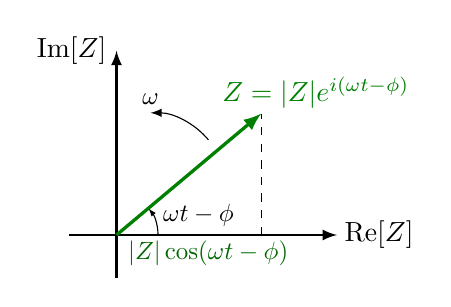
\begin{tikzpicture}
  \def\R{2.4}
  \def\ang{40}
  \coordinate (O) at (0,0);
  \coordinate (X) at (1.4*\xmax,0);
  \coordinate (Y) at (0,1.3*\ymax);
  \coordinate (R) at (\ang:\R);
  \coordinate (Rx) at ({\R*cos(\ang)},0);
  
  % AXIS
  \draw[->,thick]
    (-0.3*\xmax,0) -- (X) node[right=-1] {$\Re[Z]$};
  \draw[->,thick]
    (0,-0.3*\ymax) -- (Y) node[left] {$\Im[Z]$};
  
  % PHASOR
  \draw[dashed] (Rx) -- (R);
  \draw[vector,Rcol] (O) -- (R) node[left=16,above right=-2] {$Z = \abs{Z} e^{i(\omega t - \phi)}$};
  %\draw[vector,Rcol] (O) -- (R) node[above right=-2,scale=0.8]
  %  {$\begin{aligned}
  %     Z &= \abs{Z} e^{i(\omega t + \phi)} \\
  %       &= \abs{Z} \cos(\omega t + \phi) + \abs{Z} \sin(\omega t + \phi)
  %   \end{aligned}$};
  \node[Rcol!80!black,above=2,below right=1,scale=0.9] at (O) {$\abs{Z} \cos(\omega t - \phi)$};
  \draw pic[-sm,"$\omega t - \phi$"{scale=0.9,below=-4},draw=black,angle radius=15,angle eccentricity=2.1] {angle = X--O--R};
  \draw[->] (\ang+6:0.7*\R) arc (\ang:\ang+50:0.4*\R) node[above,scale=0.9] {$\omega$};
  
\end{tikzpicture}



% PHASOR LCR circuit
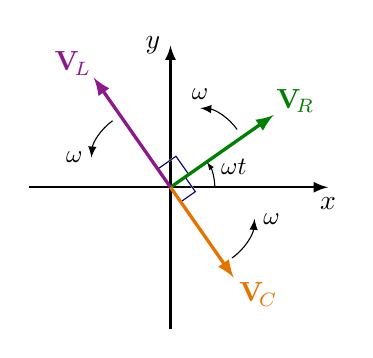
\begin{tikzpicture}
  \def\L{1.7}
  \def\R{1.6}
  \def\C{1.4}
  \coordinate (O) at (0,0);
  \coordinate (X) at (\xmax,0);
  \coordinate (Y) at (0,\ymax);
  \coordinate (C) at (\ang-90:\C);
  \coordinate (R) at (\ang:\R);
  \coordinate (L) at (\ang+90:\L);
  
  % AXIS
  \draw[->,thick]
    (0,-\ymax) -- (Y) node[left] {$y$};
  \draw[->,thick]
    (-\xmin,0) -- (X) node[below] {$x$};
  
  % PHASORS
  \rightAngle{R}{O}{C}{0.20*\R}
  \rightAngle{L}{O}{R}{0.25*\R}
  \draw[vector,Rcol] (O) -- (R) node[above right=-3] {$\VR$};
  \draw[vector,Lcol] (O) -- (L) node[above left=-3] {$\VL$};
  \draw[vector,Ccol] (O) -- (C) node[below right=-2] {$\VC$};
  \draw[->] (\ang+6:0.7*\R) arc (\ang:\ang+50:0.4*\R) node[above,scale=0.9] {$\omega$};
  \draw[->] (\ang+96:0.7*\R) arc (\ang+90:\ang+140:0.4*\R) node[left,scale=0.9] {$\omega$};
  \draw[->] (\ang-84:0.7*\L) arc (\ang-90:\ang-40:0.4*\L) node[right,scale=0.9] {$\omega$};
  \draw pic[-sm,"$\omega t$"{scale=0.9},draw=black,angle radius=16,angle eccentricity=1.5] {angle = X--O--R};
  
\end{tikzpicture}



% PHASOR LCR series circuit
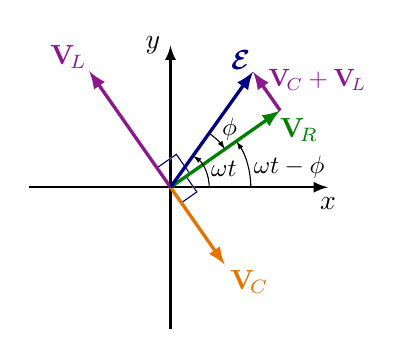
\begin{tikzpicture}
  \def\L{1.8}
  \def\R{1.7}
  \def\C{1.2}
  \def\Z{sqrt(\R^2+(\L-\C)^2)}
  \def\del{acos(\R/\Z)} %180/pi*
  \coordinate (O) at (0,0);
  \coordinate (X) at (\xmax,0);
  \coordinate (Y) at (0,\ymax);
  \coordinate (C) at (\ang-90:\C);
  \coordinate (R) at (\ang:\R);
  \coordinate (L) at (\ang+90:\L);
  \coordinate (E) at ({\ang+\del}:{\Z});
  
  % AXIS
  \draw[->,thick]
    (0,-\ymax) -- (Y) node[left] {$y$};
  \draw[->,thick]
    (-\xmin,0) -- (X) node[below] {$x$};
  
  % PHASORS
  \rightAngle{R}{O}{C}{0.20*\R}
  \rightAngle{L}{O}{R}{0.25*\R}
  \draw[vector,Lcol] (R) -- (E) node[below=3,right=2,scale=0.9] {$\VC + \VL$};
  \draw[vector,Rcol] (O) -- (R) node[left=3,below right=-1] {$\VR$};
  \draw[vector,Lcol] (O) -- (L) node[above left=-3] {$\VL$};
  \draw[vector,Ccol] (O) -- (C) node[below right=-2] {$\VC$};
  \draw[vector,Icol] (O) -- (E) node[above left=-3] {$\vb*{\EMF}$};
  %\draw pic[draw=white,line width=0.6,angle radius=14,angle eccentricity=1.45] {angle = X--O--E};
  \draw pic[-sm,"$\omega t$"{scale=0.9,below=-3},draw=black,angle radius=14,angle eccentricity=1.55]
    {angle = X--O--E};
  \draw pic[-sm,"$\omega t - \phi$"{scale=0.9,below=-1},draw=black,angle radius=29,angle eccentricity=1.55]
    {angle = X--O--R};
  \draw pic[sm-,"$\phi$"{scale=0.9},draw=black,angle radius=24,angle eccentricity=1.25]
    {angle = R--O--E};
  
\end{tikzpicture}



% PHASOR LCR parallel circuit current
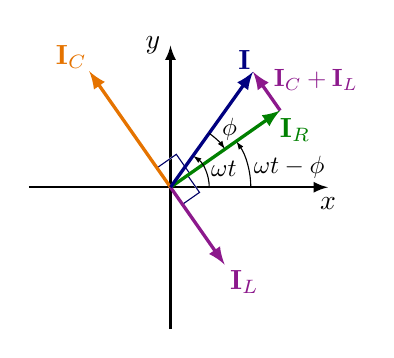
\begin{tikzpicture}
  \def\L{1.2}
  \def\R{1.7}
  \def\C{1.8}
  \def\Z{sqrt(\R^2+(\L-\C)^2)}
  \def\del{acos(\R/\Z)} %180/pi*
  \coordinate (O) at (0,0);
  \coordinate (X) at (\xmax,0);
  \coordinate (Y) at (0,\ymax);
  \coordinate (C) at (\ang+90:\C);
  \coordinate (R) at (\ang:\R);
  \coordinate (L) at (\ang-90:\L);
  \coordinate (E) at ({\ang+\del}:{\Z});
  
  % AXIS
  \draw[->,thick]
    (0,-\ymax) -- (Y) node[left] {$y$};
  \draw[->,thick]
    (-\xmin,0) -- (X) node[below] {$x$};
  
  % PHASORS
  \rightAngle{C}{O}{R}{0.25*\R}
  \rightAngle{R}{O}{L}{0.22*\R}
  \draw[vector,Lcol] (R) -- (E) node[below=3,right=4,scale=0.9] {$\IC + \IL$};
  \draw[vector,Rcol] (O) -- (R) node[left=3,below right=-1] {$\IR$};
  \draw[vector,Lcol] (O) -- (L) node[below right=-2] {$\IL$};
  \draw[vector,Ccol] (O) -- (C) node[above left=-3] {$\IC$};
  \draw[vector,Icol] (O) -- (E) node[above left=-3] {$\vb{I}$};
  \draw pic[-sm,"$\omega t$"{scale=0.9,below=-3},draw=black,angle radius=14,angle eccentricity=1.55]
    {angle = X--O--E};
  \draw pic[-sm,"$\omega t - \phi$"{scale=0.9,below=-1},draw=black,angle radius=29,angle eccentricity=1.55]
    {angle = X--O--R};
  \draw pic[sm-,"$\phi$"{scale=0.9},draw=black,angle radius=24,angle eccentricity=1.25]
    {angle = R--O--E};
  
\end{tikzpicture}



% PHASOR LCR triangle
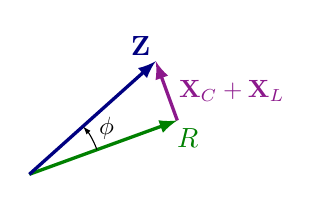
\begin{tikzpicture}
  \def\ang{20}
  \def\L{1.2}
  \def\R{2.0}
  \def\C{2.0}
  \def\Z{sqrt(\R^2+(\L-\C)^2)}
  \def\del{acos(\R/\Z)}
  \coordinate (O) at (0,0);
  \coordinate (X) at (\xmax,0);
  \coordinate (Y) at (0,\ymax);
  \coordinate (R) at (\ang:\R);
  \coordinate (Z) at ({\ang+\del}:{\Z});
  
  % PHASORS
  \draw[vector,Lcol] (R) -- (Z) node[midway,right=1,scale=0.9] {$\vb{X}_C + \vb{X}_L$};
  \draw[vector,Rcol] (O) -- (R) node[left=3,below right=-1] {$R$};
  \draw[vector,Icol] (O) -- (Z) node[above left=-2] {$\vb{Z}$};
  \draw pic[-sm,"$\phi$"{scale=0.9},draw=black,angle radius=26,angle eccentricity=1.25] {angle = R--O--Z};
  
\end{tikzpicture}




\end{document}
